\documentclass[14pt, a4paper]{article}

%Пакеты для русского  языка
\usepackage[T1,T2A]{fontenc}
\usepackage[utf8]{inputenc}
\usepackage[russian]{babel}

%Пакет расширенной математики
\usepackage{amsmath}
\usepackage{amsfonts}

%Графический пакет
\usepackage{pgfplots}
\usepackage{circuitikz}
\ctikzset{resistor = european}
\usetikzlibrary{arrows}

\pgfplotsset{compat = newest, width=77mm}
\usetikzlibrary{positioning, arrows.meta}
\usepgfplotslibrary{fillbetween}
\usepackage{subfig}

%Пакеты для отступов
\usepackage{geometry}
\geometry{top=20mm, right=15mm, bottom=20mm, left=15mm}
\usepackage{indentfirst}

%Пакет для расширенных таблиц
\usepackage{array}
\usepackage{multirow}

%Гиперссылки
\usepackage{hyperref}
\definecolor{linkcolor}{HTML}{799B03} % цвет ссылок
\definecolor{urlcolor}{HTML}{799B03} % цвет гиперссылок
\hypersetup{pdfstartview=FitH,  linkcolor=linkcolor,urlcolor=urlcolor, colorlinks=true}

%Всевозможные картинки
\usepackage{wrapfig}
\usepackage{graphicx}
\usepackage{mathtext}
\usepackage{amsmath}
\usepackage{siunitx}
\usepackage{rotating}
\usepackage{graphicx,xcolor}

\graphicspath{{pictures/}}
\begin{document}

\begin{titlepage}
    \begin{center}
    
    \Large МОСКОВСКИЙ ФИЗИКО-ТЕХНИЧЕСКИЙ ИНСТИТУТ \\ (НАЦИОНАЛЬНЫЙ ИССЛЕДОВАТЕЛЬСКИЙ УНИВЕРСИТЕТ)
    \vspace{0.3cm}
    
    \Large Физтех-школа радиотехники и компьютерных технологий
    \vspace{1cm}

  \begin{figure}[h]
    \centering
    
\includegraphics[width=0.5\linewidth]{logo.png}
    \label{fig:logo} 
  \end{figure}

    \Huge {\bfseries Лабораторная работа № 4.2.3} 
    
ИНТЕРФЕРОМЕТР РЕЛЕЯ

    \vspace{1cm}
    
    \begin{flushright}
{\LARGE Авторы:\\ Голенских Никита \\ гр. Б01-205}
\end{flushright}
    
    \vspace{\fill}
    \Large Долгопрудный 2024
    
    \end{center}
    \end{titlepage}

    \tableofcontents
    \newpage
    
\section{Аннотация}

\subsection{Цель работы} 

	Ознакомление с интерференцией на двух щелях, устройством и принципом действия интерферометра Релея и с его применением для измерения показателей преломления газов.

\subsection{Оборудование}

	Технический интерферометр ИТР-1, светофильтр, баллон с CO$_2$, сильфон, манометр, краны.

\section{Теоретическая часть}

\subsection{Зависимость показателя преломления газа от давления и температуры}

	Воспользуемся известной формулой диэлектрической проницаемости $\varepsilon$ для газа невзаимодействующих диполей: 

$$\varepsilon = n^2 = 1 + 4\pi N \alpha$$ 
где $N$ -- концентрация молекул, $\alpha$ -- поляризуемость молекулы (в ед. СГС). Эта формула справедлива для разреженных газов, и коэффициент преломления их мало отличается от единицы. Считая для разности показателей преломления $\delta n = n_2 - n_1$, измеряемой с помощью интерферометра Релея, и разности давлений $\delta P$, измеряемой с помощью манометра, с учетом зависимости давления $P$ газа от температуры $P = NkT$ , где $k$ — константа Больцмана, имеем простые соотношения: 

\begin{equation}
n-1 = 2\pi\alpha\frac{P}{kT}\:\:\rightarrow\:\: \delta n = \frac{2\pi\alpha}{kT}\delta P \text{  ,  } \frac{n_0 - 1}{n-1} = \frac{T}{T_0}\frac{P_0}{P}
\label{1}
\end{equation}

\subsection{Экспериментальная установка}

	Интерферометр Релея — прибор для измерения разности показателей преломления — основан на явлении дифракции света на двух параллельных щелях. Схема прибора представлена на рис. 1 в вертикальной и горизонтальной проекциях. Лампа накаливания Л с помощью конденсора K  освещает узкую входную щель S, расположенную в фокусе объектива O1 (фокусное расстояние $f$). Коллиматор, состоящий из щели S и объектива O1, посылает параллельный пучок на диафрагму D с двумя вертикальными щелями (расстояние между щелями d). Свет после двойной щели проходит кювету L, состоящую из двух одинаковых стеклянных камер, в которые вводятся исследуемые газы (в нашей установке — CO2 или воздух). Кювета занимает только верхнюю часть пространства между объективами O1 и O2, длина кюветы l. За кюветой расположены две стеклянные пластинки J (компенсатор Жамена, см. ниже) и пластинка П.

\begin{figure}[h]
    \centering
    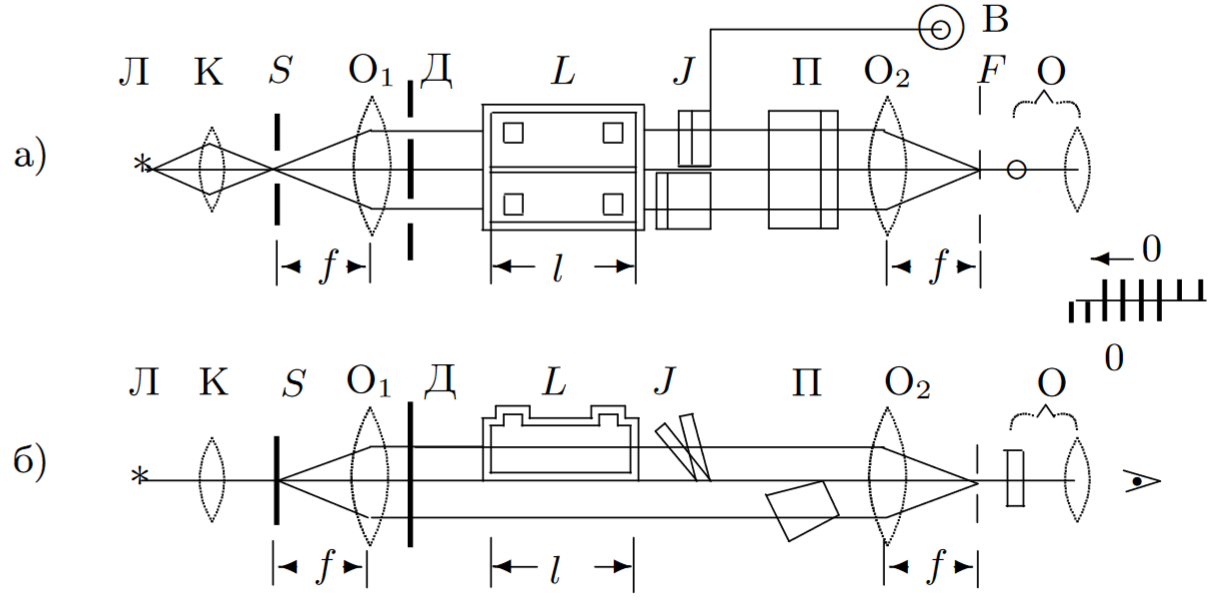
\includegraphics[width=0.9\linewidth]{expsc.png}
    \caption{Схема установки: а) вид сверху, б) вид сбоку}
    \label{fig:mpr} 
  \end{figure}
  
	Интерференционная картина (картина дифракции на двух щелях), наблюдаемая в фокальной плоскости F объектива O2, представляет собой две системы равноотстоящих полос, параллельных щелям: верхняя (подвижная) образована лучами, прошедшими через кювету, нижняя (неподвижная) — лучами, прошедшими под кюветой. Обе системы интерференционных полос разграничены при помощи пластины П тонкой разделительной линией. Для наблюдения двух систем полос в окуляре применена цилиндрическая линза диаметром 2,2 мм, ось которой расположена вертикально. Вторая («глазная») линза окуляра — обычная сферическая. Она служит для подстройки чёткости картины под глаз наблюдателя.

	При малых дифракционных углах $\varphi = \lambda / d$ расстояние между соседними светлыми (или тёмными) полосами $\delta y$ зависит от длины волны $\lambda$, фокусного расстояния $f$ объектива O2 и расстояния между дифракционными щелями $d$:

\begin{equation}
	\delta y = f \frac{\lambda}{d}
\end{equation}

	В техническом интерферометре ИТР-1, который используется в нашей работе, $f \approx 20$ см, $d \approx 1,5$ см, и $\delta y$ оказывается порядка $10^{-3}$ см. Для наблюдения таких мелких интерференционных полос требуется окуляр с большим увеличением ($\gamma \approx 150^\times$). Короткофокусная цилиндрическая линза окуляра O сильно растягивает интерференционную картину по горизонтали, не меняя её вертикальных размеров и тем самым мало ослабляя освещённость полос. Изображение светящейся точки в фокальной плоскости объектива O2 при рассматривании через цилиндрическую линзу имеет вид светлой вертикальной линии, длина которой определяется диаметром объектива. Поэтому распределение освещённости в нижней части светлой линии зависит от действия нижней части объектива, а в верхней части линии — от верхней части объектива. Таким образом, наблюдатель видит две системы полос: верхняя образована лучами, прошедшими через кюветы, нижняя — лучами, прошедшими под кюветами.

	При заполнении камер газами с одинаковым показателем преломления $n$ обе системы полос совпадают. Оптическая разность хода $\Delta = \delta n \cdot l$, возникающая при прохождении света через камеры с разными газами $\delta n = n_2 - n_1$, ведёт к поперечному смещению верхней дифракционной картины относительно неподвижной нижней. Смещение на одну полосу соответствует дополнительной разности хода $\Delta - \lambda$. Просчитав число полос $m$ между центрами обеих картин, можно рассчитать

\begin{equation}
\delta n = \frac{\Delta}{l} = m\frac{\lambda}{l}
\label{delta_n}
\end{equation}
Для точного измерения разности хода используется компенсатор Жамена (J на рис. 1) — устройство, которое позволяет вернуть подвижную систему полос к первоначальному положению, т. е. вновь совместить обе системы полос. В установке компенсатор Жамена расположен за кюветой. Он состоит из двух одинаковых плоскопараллельных стеклянных пластинок, установленных на пути лучей под углом 45$^\circ$ к горизонтали. Вращение одной из пластин вокруг горизонтальной оси, перпендикулярной оси системы, вызывает увеличение или уменьшение оптической длины пути соответствующего луча. Ось вращения снабжена рычагом, конец которого смещается при помощи микрометрического винта B.

	Интерферометр Релея можно применять для измерения небольших изменений показателей преломления жидкостей или газов, а также для определения примесей различных газов в воздухе (например, для измерения концентрации рудничного газа в шахте). Показатель преломления $n$ исследуемого газа определяется путём сравнения с воздухом при атмосферном давлении:

\begin{equation}
n = n_{air} + \frac{\Delta}{l}
\label{co2}
\end{equation}

	Для определения величины $\Delta$ компенсатор следует прокалибровать.

\newpage
\section{Ход работы}

\subsection{Условия проведения работы}

Температура в лаборатории: $T = (22.5\pm0.1) + 273.2 = 295.7 \pm 0.1$ К

Атмосферное давление на момент проведения работы: $P_{\text{атм}} = (101.8 \pm 0.1)\cdot 10^3$ Па

\subsection{Калибровка компенсатора}

Длина кюветы $l = 10 \,\text{см}$.

Прокалибруем установку в единицах $\lambda$ ($\lambda_{\text{фильтр}} = 620-720$ нм). Для этого построим график смещения от номера полосы ($m>0$ соответствует полосам справа, $m<0$ -- слева):
	
\begin{table}[!ht]
    \centering
    \caption{Калибровка компенсатора: $z(m)$}
    \begin{tabular}{|c|c|c|c|c|c|c|c|c|c|c|}
    \hline
        $m$ & 0 & 1 & 2 & 3 & 4 & 5 & 6 & 7 & 8 & 9  \\ \hline
        $z$, мм & 3,18 & 3,52 & 3,85 & 4,18 & 4,51 & 4,82 & 5,12 & 5,47 & 5,8 & 6,12  \\ \hline
        $m$ & 0 & -1 & -2 & -3 & -4 & -5 & -6 & -7 & -8 &   \\ \hline
        $z$, мм & 3,18 & 2,85 & 2,52 & 2,21 & 1,9 & 1,59 & 1,27 & 0,95 & 0,63 &   \\ \hline
    \end{tabular}
    \label{calibr}
\end{table}

\begin{figure}[h!]
		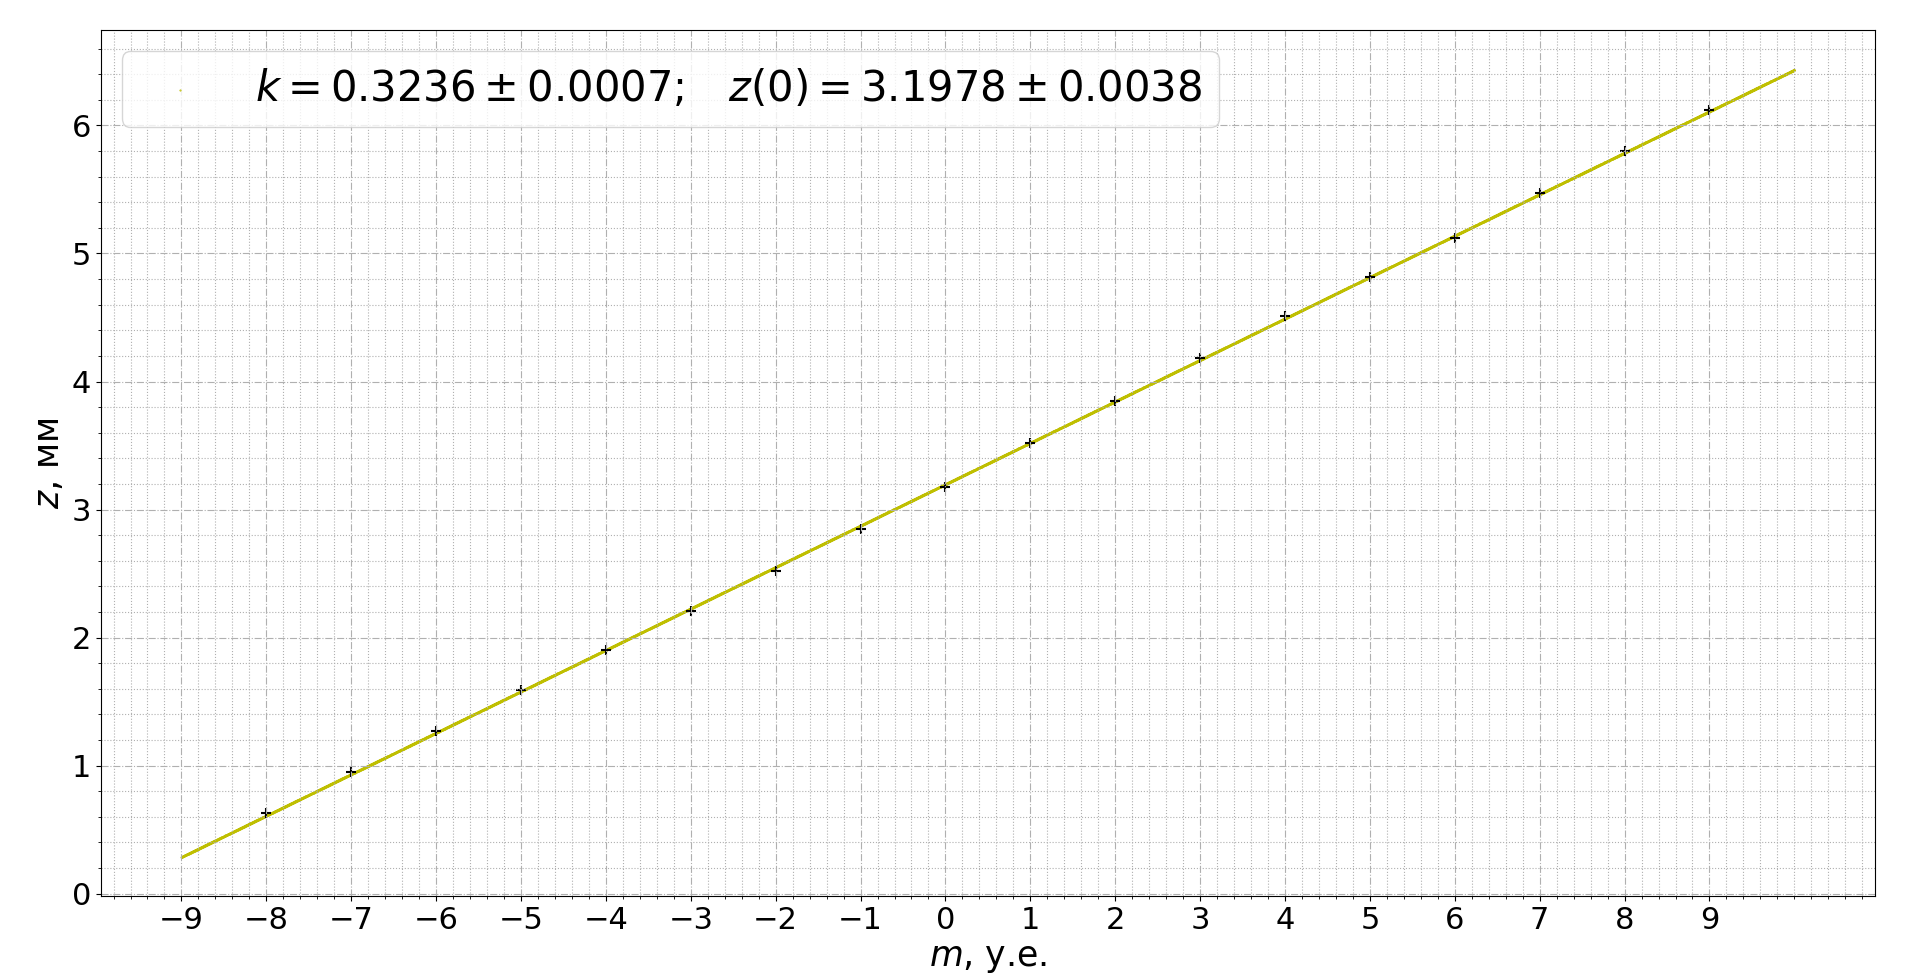
\includegraphics[width = 1.03\linewidth]{graph1.png}
		\caption{Зависимость смещения от номера полосы интерференционной картины}
\end{figure}

Из полученного графика получаем, что 
$$z = (0.3236 \pm 0.0007)\cdot m \pm (3.1978 \pm 0.0038) $$

Отметим, что рассчитанный угловой коэффициент получен для определенного промежутка значений $\lambda$. В дальнейшем  будем считать $\lambda = 670 \pm 50$ нм, ($\varepsilon \approx 8\%$). Любые другие погрешности малы, по сравнению с этой.

\newpage
\subsection{Зависимость $\delta n$ от давления для воздуха}

Изменяя давление в кювете, фиксируем смещение интерференционной картины, относительно исходного положения.

\begin{table}[!ht]
    \centering
    \caption{Зависимость смещения интерференционной картины от давления: $z(\Delta(P)$}
    \begin{tabular}{|c|c|c|c|c|c|c|c|c|c|}
    \hline
        $\Delta P$, мм вод. ст. & -800 & -700 & -600 & -500 & -400 & -300 & -200 & -100 & 0  \\ \hline
        $z$, мм & 2 & 2,21 & 2,33 & 2,48 & 2,62 & 2,78 & 2,87 & 3,02 & 3,18  \\ \hline\hline
        $\Delta P$, мм вод. ст. & 100 & 200 & 300 & 400 & 500 & 600 & 700 & 800 & 900  \\ \hline
        $z$, мм & 3,39 & 3,5 & 3,64 & 3,74 & 3,9 & 4,04 & 4,19 & 4,33 & 4,46  \\ \hline
    \end{tabular}
\end{table}

Воспользуемся калибровочным графиком \ref{calibr} (его угловым коэффициентом) и формулой \ref{delta_n} для нахождения зависимости $\delta n (\Delta P)$.

\begin{figure}[h!]
		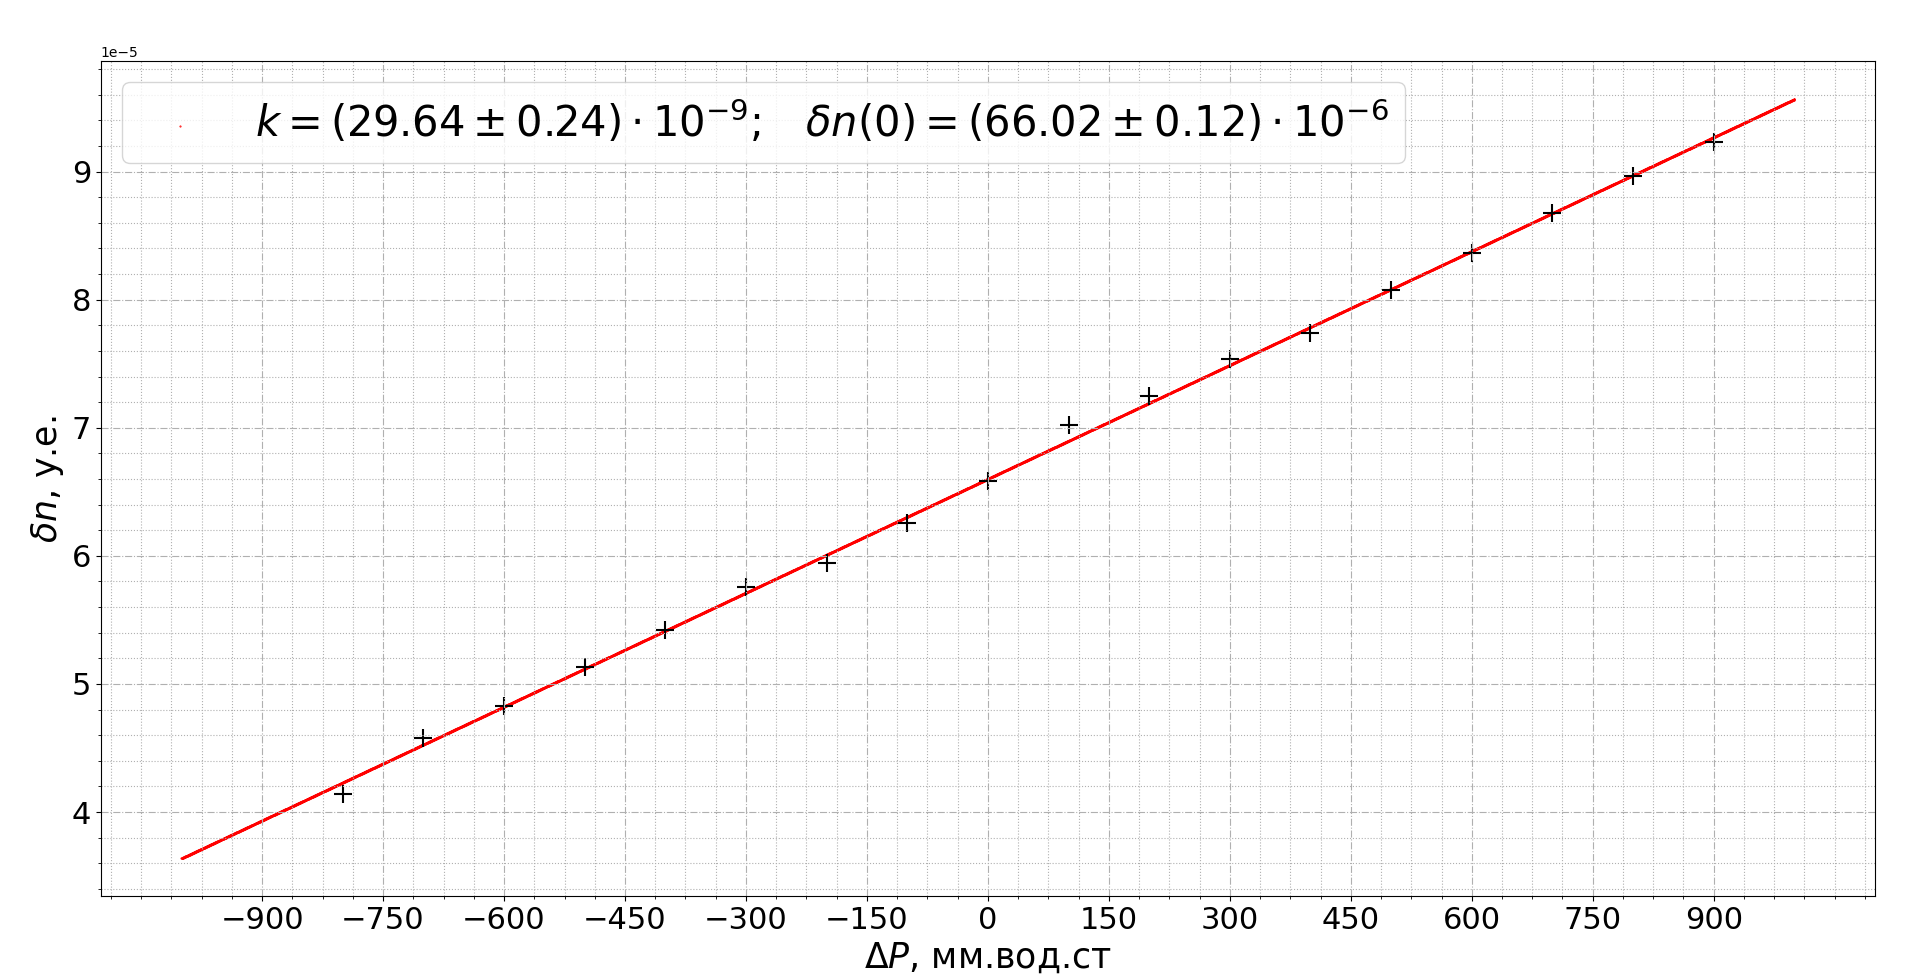
\includegraphics[width = 1.03\linewidth]{graph2.png}
		\caption{Зависимость смещения от номера полосы интерференционной картины}
\end{figure}

Таким образом, получаем:
$$\delta n = (29.64 \pm 0.24)\cdot10^{-9}\cdot\Delta P + (66.02\pm0.12)\cdot10^{-6}$$

Определим поляризуемость "молекул воздуха" с помощью формулы \ref{1} ( [1 мм вод. ст.] = [9,81 Па] ) и с учетом погрешности длины волны.

$$\alpha = \frac{\delta n}{\Delta P} \cdot 2k_bT = (2.47 \pm 0.22)\cdot 10^{-29}, \;\;\;\; \varepsilon \approx 9 \%  $$

Рассчитаем показатель преломления воздуха:

$$n = 1 + \frac{\alpha P}{2k_bT} = 1.000308 \pm 0.000028, \;\;\;\; \varepsilon \approx 9 \%$$

Полученное значение хорошо сходится с табличным ($n^\text{табл}_{возд} \approx 1.0003$)
\newpage
\subsection{Определение показателя преломления углекислого газа}

Заполним кювету углекислым газом и пронаблюдаем зависимость смещения компенсатора от времени.

%таблица и график
\begin{figure}[h!]
		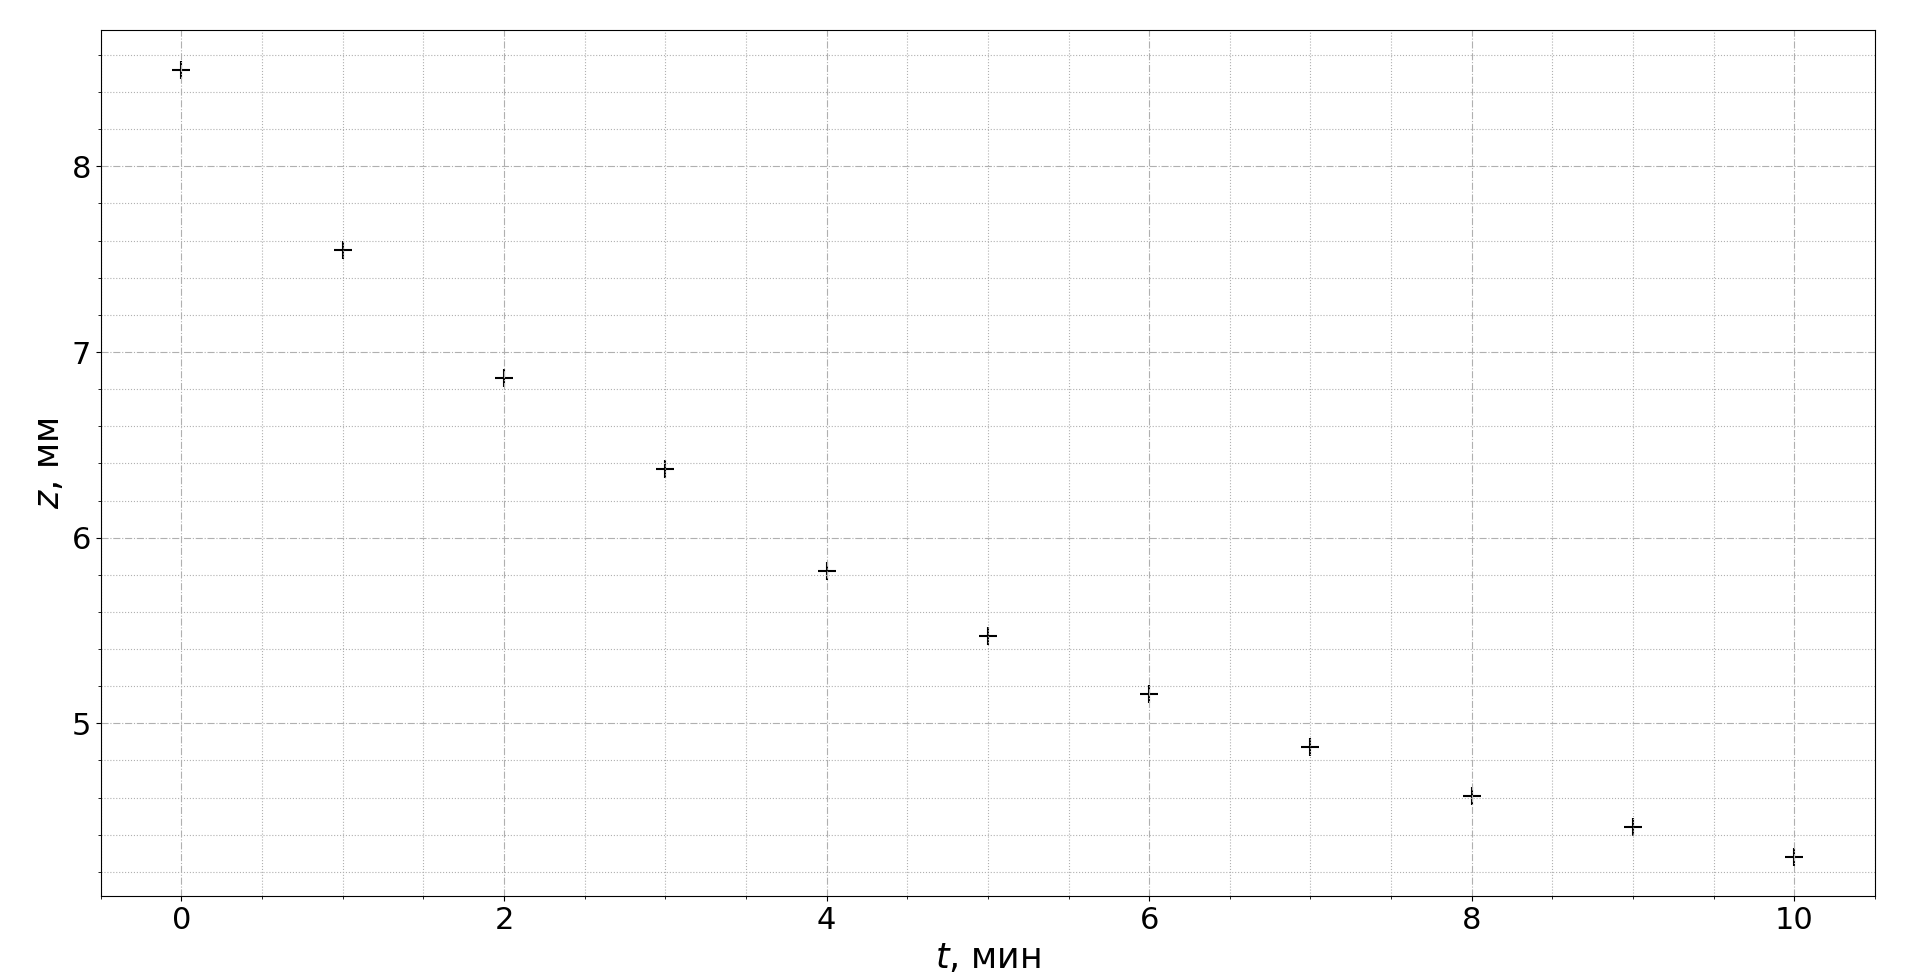
\includegraphics[width = 1.03\linewidth]{co2.png}
		\caption{Зависимость смещения интерференционной картины CO$_2$ от времени}
\end{figure}

Таким образом, с учетом формулы \ref{co2} определим показатель преломления CO$_2$.

 $$n_{CO_2} = 1.00048 \pm 0.000057, \;\;\;\; \varepsilon \approx 12\%$$

Полученное значение хорошо сходится с табличным ($n^\text{табл}_{CO_2} \approx 1.00045$)
%пересчет для н.у. и сравнение с табличным

\section{Обсуждение результатов}

	Интерферометр Релея позволяет измерять разность показателей преломления в двух кюветах с высокой точностью. Полученные значения хорошо сходятся с табличными:
	
	 $$n = 1.000308 \pm 0.000028, \;\;\;\; \varepsilon \approx 9 \%$$
	 
	 $$n^\text{табл}_{\text{возд}} \approx 1.0003$$
	 
	 $$n^\text{эксп}_{CO_2} = 1.00048 \pm 0.000057, \;\;\;\; \varepsilon \approx 12\%$$
	 
	 $$n^\text{табл}_{CO_2} \approx 1.00045$$

	 Однако для этого нужно поддерживать давление в кюветах и концентрацию газа постоянными, в противном случае точность измерений может ухудшаться. Именно этому и была подвержена установка, ведь при изменении давления в кювете манометр заметно плыл, была необходимость действовать быстро, из-за чего возросла случайная погрешность (наибольший вклад в погрешности исследуемых величин внесла погрешность зависимости изменения показателя преломления от изменения давления для воздуха: $\varepsilon (\delta n (\Delta P)) \approx 0.8\%$ ). 
	 
	 Также следует отметить, что для определения показателя преломления любого отдельно взятого газа, крайне важно, чтобы он полностью вытеснил воздух. Для этого в нашей установке мы изолировали кювету и баллон с определенным количеством углекислого газа, с помощью нескольких заполнений баллона и, затем, кюветы, мы вытеснили воздух. Однако появилась важная проблема: газ поступал в кювету \textbf{не под атмосферным давлением}, а от манометра мы установку отключили, поэтому в первоначальный момент времени мы не знали давление и посчитали показатель преломления \textbf{приблизительно} при атмосферном давлении с неизвестной точностью. 




\end{document}